\chap{Latches, Flip-flops, and Registers}

\section{Part V}
\begin{itemize}
    \item []\textbf{REQUIREMENT} 
        \begin{enumerate}
            \item We wish to display the hexadecimal value of an 8-bit number A on the two 7-segment displays HEX3 - 2. We also wish to display the hex value of an 8-bit number B on the two 7-segment displays \textbf{HEX1 - 0}. 
            \item The values of A and B are inputs to the circuit which are provided by means of switches \textbf{SW7-0}. To input the values of A and B, first set the switches to the desired value of A, store these switch values in a register, and then change the switches to the desired value of B. Finally, use an adder to generate the arithmetic sum S = A + B, and display this sum on the 7-segment displays HEX5 - 4. Show the carry-out produced by the adder on LEDR[0].
        \end{enumerate}
    \item []\textbf{SOLUTION}
        \begin{itemize}
            \item []For this part, we use 2 different D\_latch with 1 Enable pin to store the input into A and B
                \begin{lstlisting}[language = verilog]
    D_latch     inst1 (.CLK(CLK),  .D(Num), .Q(A));
    D_latch     inst2 (.CLK(~CLK), .D(Num), .Q(B));
                \end{lstlisting}
            \item []Then, we use block sum8bits which is the combination of 2 sum4bits blocks we mentioned before, to do the sum between A and B.
                \begin{lstlisting}[language = verilog]
    sum8bits	sum	(.A(A), .B(B), .C_IN(0), .SUM(Sum), .C_OUT(C_out));            \end{lstlisting}
        \end{itemize}
    \item []\textbf{VERIFICATION}
        \begin{figure}[h]
            \centering
            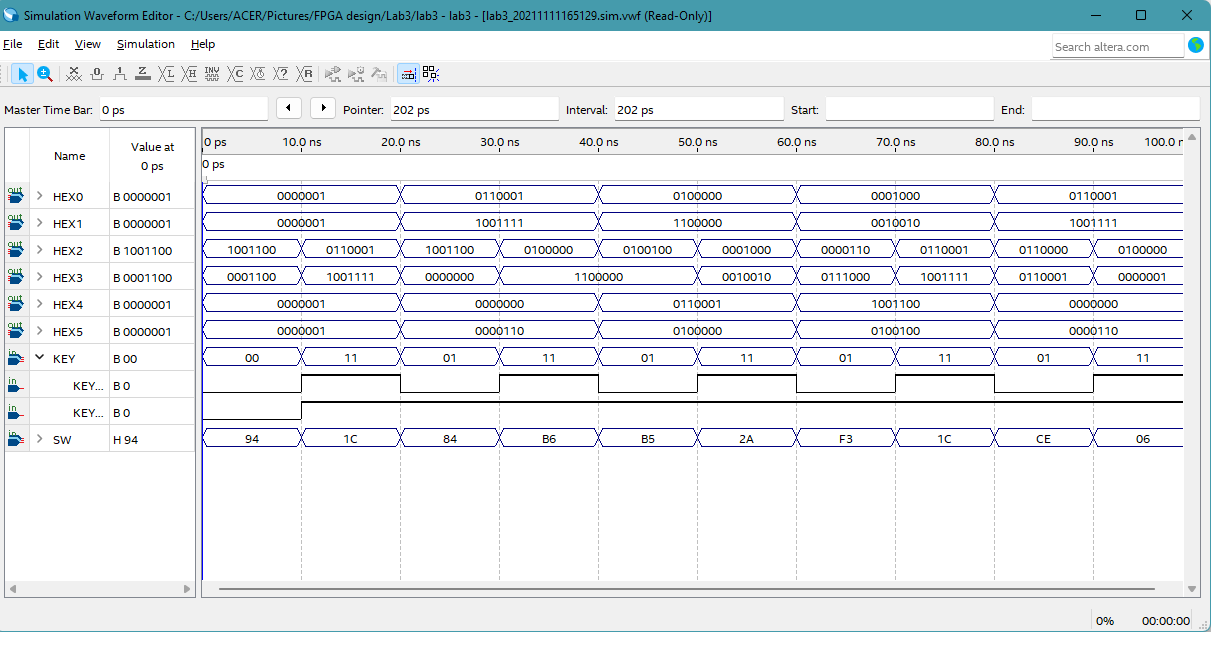
\includegraphics[scale = 0.5]{source/picture/lab3/lab3.png}
            \caption{Simulation Result}
        \end{figure}
\end{itemize}
